\chapter{Scalability}
\label{chap:Scalability}

Graph visualizations are always limited by the number of nodes, as well as the number of edges. The patterns in figure \ref{fig:patterns} can only be recognized if completely visible, therefore the whole adjacency matrix must be visible to find all of them. Otherwise, patterns may not be entirely visible. This chapter gives an overview of the scalability of adjacency matrices, by estimating the upper limit of nodes in fully visible adjacency matrix visualizations, explaining the problems of non fully visible matrix visualizations, and reviewing the implementations 'Matrix zoom' \citep{ham-ivis-2003,abello2004} and Nodetrix \citep{henry-nodetrix-2007}.


\section{Maximum number of Nodes}
A short best case estimation will show the scalability limits of fully visible adjacency matrix visualizations. Assuming all patterns should be recognizable, the whole matrix must be visible at once. Given a screen size of 25”, the number of nodes depends on the size of column, row and cell. The number of displayable edges is in adjacency matrices always $|nodes|^2$.

Size of cells, rows and columns is determined by their requirements. Pure visibility, operability, or permanently visible node labels or edge weights (cell labels) require increasingly more space.
If only a visible mark is required for an edge, one pixel is the lower limit for the mark's size, otherwise marks can not be associated to the source or destination edge. High resolution screens do not increase the maximum number of nodes, since it is getting very hard to follow the grid lines to other nodes. Therefore, more than ~3000 nodes on a screen seem to cause an unreadable visualization.

Mouse interactions like ‘on hover tooltips’ will add the option to identify source and destination nodes of an edge, but will also use more space and restrict the maximum number of nodes. This will shrink the maximum number of nodes to ~300.
If edge -- node association is an important task, permanently visible node labels in header will allow an interaction-less visualization of the graph. Additional space for labels reduces the maximum node count to 30.
 
 
\begin{table}[]
\centering
\begin{tabular}{|l|l|l|}
\hline
25" screen                 & max nodes & max edges                \\ \hline
Pixel grid                 & 3000      & $10^7$                     \\ \hline
Interactive cell or header & 300       & $10^5$                     \\ \hline
Labeled cell or header     & 30        & $10^3$                     \\ \hline
\end{tabular}
\caption
  [Upper Limit of Nodes of Adjacency Matrix]
  {Estimated Upper limit of nodes on a 25" screen for fully visible adjacency matrix visualizations.}
  \label{table_upperlimit}
\end{table}



\section{Simple Zooming}
Putting an adjacency matrix in a zoom box obviously increases the maximum number of nodes. 
When zoomed in, the readability of node and cell labels increases, but patterns may not be completely visible anymore. This requires the user to search the matrix by panning. When zoomed out, labels are not readable anymore and interactions with cells are impossible due to their small size. 

The following two section review Matrix zoom, a zoomable matrix visualization which avoids these problems for clustered graphs. A general solution, without using known additional properties of the graph like its clusters, was not found in the survey.

\section{Matrix Subdivision}

Matrix zoom is a zoomable matrix visualization tool \citep{ham-ivis-2003}. It solves the label readability problem by finding new labels for groups of nodes or edges when zoomed out. It comes with a default data set, describing a software repository. The nodes of the actual graph are function declarations and function calls of the source code, so it is the complete call graph of a software project. Classes, packages and layers are considered as clusters of the graph. 

When node labels get too small to be read, they form groups based on their containing classes, these groups are labeled with the class name. Multiple classes are represented by packages and so on. When edge marks get too small, an $n \times m$ block of edge marks is transformed to one cell, by calculating the density of the block and associating the cell color to it.

\begin{figure}[h]
\centering
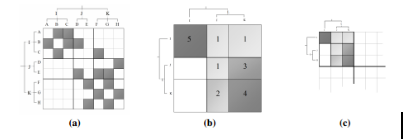
\includegraphics{images/matrixzoom_transform}
\caption
  [Cell and Header Transformations]
  {Cell and header transformations.}
  \imgcredit{Image taken from \citep{ham-ivis-2003}.}
  \label{fig:matrixzoom_transform}
\end{figure}




\subsection{Cell and Header Transformations}   
In general, this concept needs a way to transform blocks of labels to one label. The given example fits well to this requirement, since classes are packages and thus clusters and have human readable names. If the graph is clustered by algorithms, meaningful names of clusters must be found, see figure \ref{fig:matrixzoom_transform}.

If other header visualization techniques are used, the transformation must be adapted, see Chapter \ref{chap:headers}. For example, if in or out degrees are visualized in the header, the average degree might be visualized by the group.

Transforming cell blocks to a single cell can be done in various ways. If just the existence of an edge is relevant, the group cell may be rendered like an edge if at least one edge is in the cluster. Average weight, density or degree may also be relevant. Which of these transformations should be used is dependent on the requirements of the application, however, only one can be chosen.

This concept is suitable for recursive clustering, where each cluster is a zoom level. An extended version of Matrix zoom  \citep{abello2004} uses tree structures in the matrix headers for better navigation, see figure \ref{fig:matrixzoom_abello}.

\begin{figure}[h]
\centering
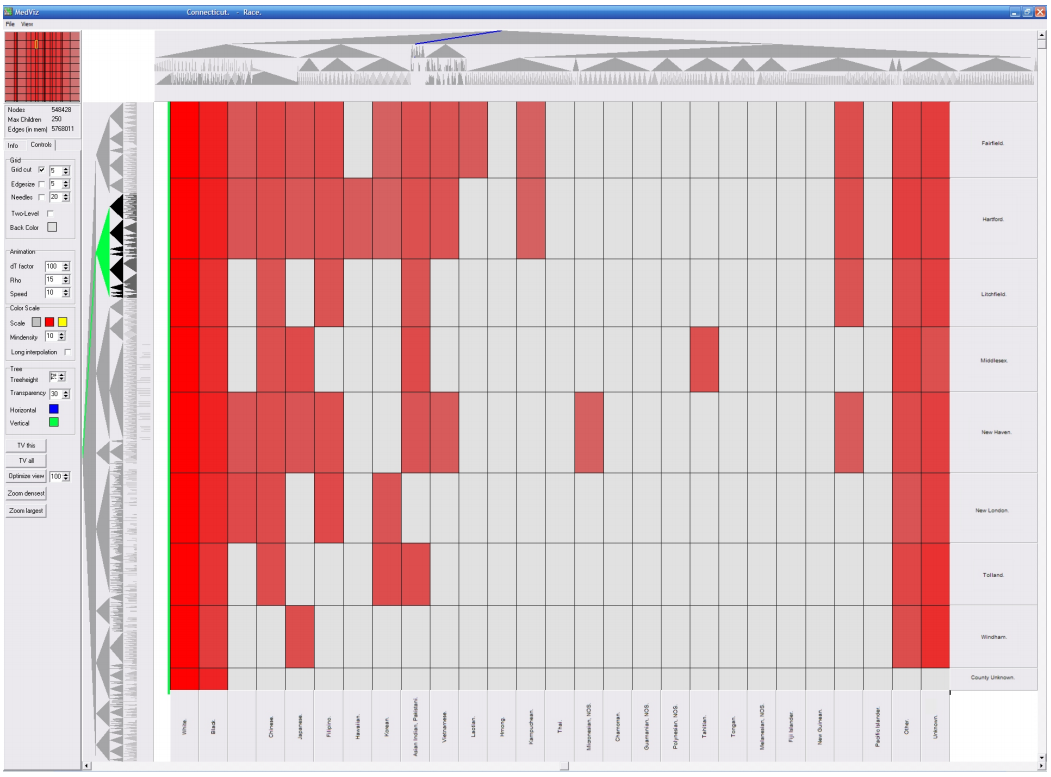
\includegraphics[width=\textwidth]{images/matrixzoom_abello}
\caption
  [Cluster Tree Visualized in Matrix Header for Better Navigation]
  {Cluster tree visualized in matrix header for better navigation.}
  \imgcredit{Image taken from Phd. thesis \citep{ham2005phd}}
  \label{fig:matrixzoom_abello}
\end{figure}





\subsection{Sorting and Clustering}   

The ‘edge mark in invisible area' problem is reduced by the clustering, since most connections are within the cluster, it is less likely to have invisible edge marks if zoomed to a cluster. See figure \ref{fig:matrixzoom_cluster}. 
The quality of this reduction depends on the chosen clustering algorithm and the sort algorithm, see figure \ref{fig:reorder}. In general the cluster algorithm is executed first, and the order algorithm is applied to the elements within the cluster, and then to the clusters themselves.

\begin{figure}[h]
\centering
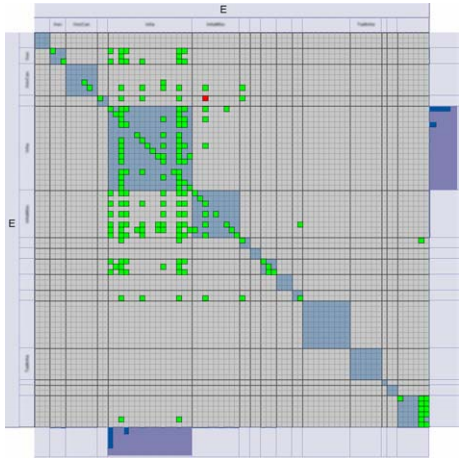
\includegraphics[width=\textwidth/2]{images/matrixzoom_cluster}
\caption
    [Typical Matrix Subdivision View of Matrix zoom]
    {Typical matrix subdivision view of Matrix zoom.}
    \imgcredit{Image taken from the Phd. thesis \citep{ham2005phd}}
    \label{fig:matrixzoom_cluster}
\end{figure}

This concept can not be applied always. In best case the data set gives a natural cluster tree like the software repository. Otherwise, a suitable cluster algorithm must be found, as well as human readable labels for those automatically generated clusters. It should be considered as data preprocessing, since it may be applied to large data sets.













\section{Hybrid Representation}
Nodetrix is a graph adjacency matrix hybrid. Adjacency matrices are better suited for dense graphs, so the idea of Nodetrix is to replace unreadable dense sub clusters in traditional graph visualizations with adjacency matrix visualizations. Figure \ref{fig:nodetrix_cluster} shows a traditional graph, with a dense green cluster. It is hard to find the nodes of an edge in the traditional view on the left. On the right side the dense sub cluster is replaced by a better readable  adjacency matrix. Edges out of the cluster are rendered as lines to the nodes in the traditional graph view, or other matrix views, and are therefore always visible \citep{henry-nodetrix-2007}.



\begin{figure}[h]
\centering
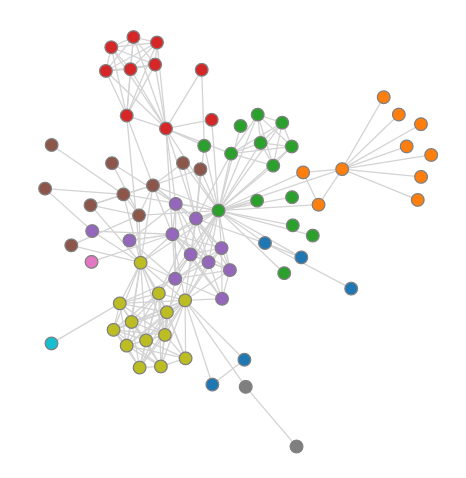
\includegraphics[width=\textwidth/3]{images/nodetrix_matrix}
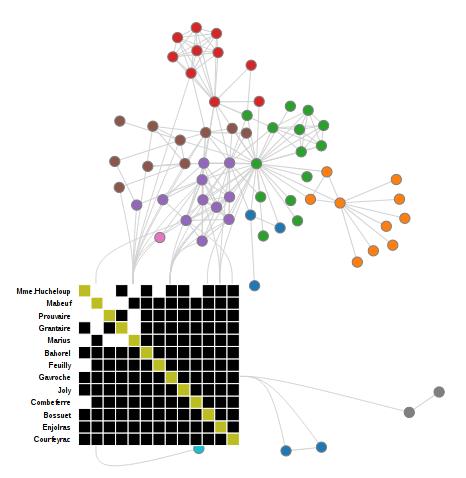
\includegraphics[width=\textwidth/3]{images/nodetrix_cluster}
\caption
  [Nodetrix with Traditional Graph View, Enhanced with Adjacency Matrix View]
  {Nodetrix with traditional graph view, enhanced with adjacency matrix view.}
  \imgcredit{Screenshot created an author of this thesis using Nodetrix \citep{henry-nodetrix-2007}}
  \label{fig:nodetrix_cluster}
\end{figure}


